% Provenance (never printed): see sources/outline_sources.md (Year 2: effusive and explosive
% eruptions, eruptive styles, eruption columns, pyroclastic deposits, explosivity index,
% volcano monitoring).
% Curves from figdata/bachelor-2/eruptions.py (closed-system gas fraction, Cotopaxi Layer 5
% thinning, GVP frequency-size law, column height fits, Mogi uplift); exercise and problem
% values in the Book 4 scratch calculators calc/ch06.py and calc/ch06pb.py.
\chapter{الثورانات البركانية}\label{ch:b2:eruptive-styles}

في 15 يونيو 1991 قذف جبل بيناتوبو في الفلبين أكثر من خمسة
كيلومترات مكعبة من المواد؛ وارتفعت سحابة رماده إلى
\qty{35}{km}، وانهارت القمّة في كالديرا عرضها \qty{2.5}{km}،
وبردت العشرون مليون طن من ثاني أكسيد الكبريت التي حقنها في الستراتوسفير
الكرةَ الأرضية كلها بنحو نصف درجة مدة سنتين. وقبل ذلك بأسبوع لم تفعل أول
صهارة بلغت السطح شيئًا من هذا: فبعد أن فقدت معظم
غازها في طريق صعودها، رشحت قبّةً من الحمم. وعلى كيلاويا، في هاواي، صبّ
ثوران بوؤو أوؤو \qty{4.4}{km^3} من الحمم، وهو حجم مماثل،
على مدى خمس وثلاثين سنة، نوافيرَ وتدفّقات دمّرت 215 مبنى
دون أن يرفع قطّ عمودًا شاهقًا من الرماد. الأرض نفسها، والفيزياء نفسها، وثلاثة سلوكات: وما
يفصل بينها هو كمية الغاز التي تحملها \omterm{def:b2:magma-emplacement:magma}{الصهارة}، وهل يستطيع ذلك الغاز أن يغادر
المصهور بهدوء، ومدى سرعة صعود \omterm{def:b2:magma-emplacement:magma}{الصهارة}. يتتبّع هذا الفصل الثوران
من الفقاعات في القناة إلى العمود فوق المنفذ والرواسب التي
يخلّفها، ثم يقيس الثورانات ويعدّها، ويراقب البراكين بحثًا عن
العلامات التي تنبئ بقدوم أحدها.
% ledger: usgs:pinatubo-1991, usgs:puuoo

\begin{recall}
\textbf{من المجلدات المدرسية}: البركان، ومنفذه وفوّهته، والحجرة الصهارية
تحته، والحمم، والرماد البركاني. \textbf{من
\cref{ch:b2:magma-emplacement}}: \omterm{def:b2:magma-emplacement:volatiles}{المكوّنات الصهارية المتطايرة}، وانفصالها تحت
ضغط الإشباع، وقانون الجذر التربيعي لذوبانية الماء $w = s\sqrt p$ مع
$s \approx 0.34$ في المئة لكل $\sqrt{\unit{MPa}}$ للبازلت و$0.44$
للريوليت، ولزوجات المصاهير، التي يفصل بينها عشر رتب من القيمة.
\textbf{من كتب الفيزياء}: قانون الغاز المثالي $pV = nRT$؛ والطفو؛
والتحليل البعدي، الذي يبني التركيبة الوحيدة من المقادير المعطاة
التي لها بُعد الجواب؛ ومدى المقذوف، $v^2\sin 2\theta/g$
دون مقاومة الهواء. \textbf{من كتب الرياضيات}: عملية بواسون،
التي تعطي فيها أحداث مستقلة بمعدل ثابت $\lambda$ حدثًا واحدًا على الأقل
في زمن $t$ باحتمال $1 - e^{-\lambda t}$؛ ومستقيمات المربعات الصغرى.
ومن مجلد السنة الأولى: الزلازل ومقاديرها.
\end{recall}

\section{انسيابي أم انفجاري}

\begin{definition}[الثورانات الانسيابية والانفجارية، التفتّت]\label{def:b2:eruptive-styles:regimes}
\emph{الثوران الانسيابي}\index{الثوران الانسيابي} ثوران يغلب عليه
تدفّق الحمم، التي تجري بعيدًا عن المنفذ سائلًا متماسكًا.
و\emph{الثوران الانفجاري}\index{الثوران الانفجاري} ينتج أساسًا قطعًا،
رمادًا وخفافًا وحطامًا مقذوفًا، يحملها غاز متمدّد. و\emph{تفتّت
الصهارة}\index{تفتّت الصهارة} هو تحوّل مصهور متصل
يحوي فقاعات إلى غاز متصل يحمل قطرات وقطعًا من المصهور؛
وهو يحوّل تدفّقًا انسيابيًا إلى تدفّق انفجاري.
\end{definition}
% ledger: usgs:glossary-ch6, cassidy18:fragmentation

الغاز هو ما يدفع هذا الانتقال. \omterm{def:b2:magma-emplacement:magma}{فالصهارة} الصاعدة من العمق تحمل
ماءً وثاني أكسيد كربون مذابين؛ وتحت ضغط إشباعها تخرج المكوّنات المتطايرة
من المحلول فقاعات، وتتمدّد الفقاعات كلما انخفض الضغط.
فإن بقيت في المصهور، سرعان ما يملأ الغاز معظم الحجم.

\begin{proposition}[الكسر الحجمي للغاز في نزع الغاز في نظام مغلق]\label{prop:b2:eruptive-styles:gas}
لتحوِ صهارةٌ كسرًا كتليًا $w_0$ من الماء، ذوبانيته $w(p) =
s\sqrt p$، ولنفترض أن الماء المنفصل يبقى مع المصهور غازًا مثاليًا
عند درجة الحرارة $T$. تحت ضغط الإشباع $p_s = (w_0/s)^2$، يحوي الكيلوغرام
الواحد من \omterm{def:b2:magma-emplacement:magma}{الصهارة} $x = w_0 - s\sqrt p$ كيلوغرامًا من البخار، ويكون الكسر
الحجمي للغاز
\[
\phi(p) = \frac{V_g}{V_g + V_m}, \qquad V_g = \frac{x\,RT}{M p}, \qquad
V_m = \frac{1 - x}{\rho_m},
\]
حيث $M = \qty{0.018}{kg/mol}$ الكتلة المولية للماء و$\rho_m$ كثافة
المصهور.
\end{proposition}

\begin{proof}
فوق $p_s$ يستطيع المصهور أن يحمل كل مائه ولا يوجد غاز. وتحت $p_s$
لا يحتفظ المصهور إلا بذوبانيته $s\sqrt p$، فتكون كتلة $x = w_0 - s\sqrt p$ لكل
كيلوغرام من \omterm{def:b2:magma-emplacement:magma}{الصهارة} بخارًا. ويشغل هذا البخار، أي $x/M$ مولًا، الحجم $xRT/(Mp)$ حسب
قانون الغاز المثالي؛ ويشغل الباقي من المصهور، أي $1 - x$ كيلوغرامًا، الحجم $(1 - x)/\rho_m$.
ومن ذلك يتبع الكسر الحجمي.
\end{proof}
% ledger: moore98:h2o

لأن $V_g$ ينمو بنسبة $1/p$، تنتفخ الرغوة أسرع ما يكون قرب السطح.
ويتتبّع الشكل أدناه ريوليتًا فيه \qty{5}{\percent} من الماء وبازلتًا
فيه \qty{1}{\percent}. يتشبّع الريوليت عند \qty{127}{MPa}، أي على عمق نحو
\qty{5}{km}؛ وعند \qty{10}{MPa} يملأ غازه \qty{82}{\percent} من
الحجم. وفي نموذج منشور لجريان القناة تتفتّت \omterm{def:b2:magma-emplacement:magma}{الصهارة} حين يملأ
الغاز \qty{85}{\percent} من حجمها، وهو مستوى يبلغه هذا الريوليت عند
\qty{8.2}{MPa}، أي على نحو \qty{330}{m} تحت المنفذ لتدرّج ضغط قدره
\qty{0.025}{MPa/m}. أمّا البازلت فلا يتشبّع إلا عند \qty{8.7}{MPa} ويبلغ
الرغوة نفسها عند \qty{1.8}{MPa}، في حدود مئة متر من السطح.
% ledger: cassidy18:fragmentation, cassidy18:ascent

\begin{omfigure}
\centering
\begin{tikzpicture}
\begin{axis}[omrecord, width=0.82\linewidth, height=5.6cm, xmode=log,
  xmin=0.01, xmax=200, ymin=0, ymax=1,
  xlabel={\foreignlanguage{arabic}{الضغط \babelsublr{(\unit{MPa})}}}, ylabel={\foreignlanguage{arabic}{الكسر الحجمي للغاز $\phi$}},
  legend pos=south west, legend style={font=\scriptsize},
  tick label style={font=\scriptsize}, label style={font=\small}]
\addplot[very thick, red!70!black] table[x=p_MPa, y=rhyolite] {figdata/out/bachelor-2-eruptions-gas.dat};
\addlegendentry{\foreignlanguage{arabic}{ريوليت، \qty{5}{\percent} من H$_2$O، \qty{850}{\celsius}}}
\addplot[very thick, black, dashed] table[x=p_MPa, y=basalt] {figdata/out/bachelor-2-eruptions-gas.dat};
\addlegendentry{\foreignlanguage{arabic}{بازلت، \qty{1}{\percent} من H$_2$O، \qty{1200}{\celsius}}}
\draw[densely dotted, thick, gray] (axis cs:0.01,0.85) -- (axis cs:200,0.85);
\node[anchor=north west, font=\scriptsize, inner sep=1pt] at (axis cs:0.012,0.835) {التفتّت في نموذج للقناة};
\end{axis}
\end{tikzpicture}
\par\smallskip{\small الكسر الحجمي لبخار الماء المنفصل بدلالة الضغط
في نزع الغاز في نظام مغلق (\cref{prop:b2:eruptive-styles:gas})، مع قوانين
الذوبانية في \cref{ch:b2:magma-emplacement}. ينخفض الضغط نحو اليسار، كلما
صعدت \omterm{def:b2:magma-emplacement:magma}{الصهارة}؛ ويحدّد الخط المنقّط كسر الغاز الذي يفتّت عنده نموذج
منشور للقناة \omterm{def:b2:magma-emplacement:magma}{الصهارة}.}
\end{omfigure}
% ledger: moore98:h2o, cassidy18:fragmentation

فالبازلت يتفتّت هو الآخر، لو بقي غازه فيه؛ وفي نافورة الحمم
الهاوايية يحدث ذلك فعلًا، قرب المنفذ. وما يجعل معظم الثورانات البازلتية معتدلة هو أن
الغاز لا يلزمه البقاء. ففي مصهور منخفض اللزوجة تصعد الفقاعات عبر
السائل، وتندمج وتفلت، وما إن تتصل الفقاعات في شبكة نفوذة،
وهو ما يحدث عند كسور غازية بين \qty{30}{\percent} و\qty{78}{\percent}
في التجارب، حتى يتسرّب الغاز عبر الجدران والمنفذ دون أن يحمل
المصهور معه: فتنزع \omterm{def:b2:magma-emplacement:magma}{الصهارة} غازها في نظام مفتوح وتبلغ السطح
حممًا. أمّا \omterm{def:b2:magma-emplacement:magma}{الصهارة} اللزجة فتحتفظ بفقاعاتها وتتفتّت بدلًا من ذلك، إذ ينكسر المصهور
كالزجاج حين يُمطّ أسرع مما يستطيع أن يجري. ومعدل الصعود يحسم
بين الاثنين بقدر ما يحسم التركيب: فعبر ثورانات كثيرة، يقترن النشاط الانسيابي
بمعدلات انخفاض ضغط قرب \qty{0.0001}{MPa/s} \omterm{def:b2:eruptive-styles:regimes}{والثورانات الانفجارية}
بمعدلات قرب \qty{1}{MPa/s}، ويمكن لتغيّر في لزوجة المصهور بمقدار نصف
وحدة لوغاريتمية، أي بعامل ثلاثة تقريبًا، أن يقلب الثوران من نظام إلى
آخر. وكانت \omterm{def:b2:eruptive-styles:dome}{قبّة الحمم} الأولى في بيناتوبو وثورانه الذروي بعد أسبوع
من \omterm{def:b2:magma-emplacement:magma}{الصهارة} نفسها: فالدفعة الأولى كان لديها وقت لتفقد غازها، والتالية لم يكن.
% ledger: cassidy18:fragmentation, cassidy18:ascent, usgs:pinatubo-1991

الماء الآتي من الخارج يفعل ما يفعله غاز \omterm{def:b2:magma-emplacement:magma}{الصهارة} نفسه. فالمياه الجوفية أو البحيرة أو
البحر إذا لاقت \omterm{def:b2:magma-emplacement:magma}{الصهارة} تتحوّل فجأة إلى بخار، ويحطّم تمدّد الماء
المحمّص \omterm{def:b2:magma-emplacement:magma}{الصهارة}: وتُظهر التجارب أن أكثر من \qty{30}{\percent} من
الحرارة المتاحة يمكن أن يتحوّل إلى طاقة ميكانيكية. وعندئذ يمكن حتى لصهارة فقيرة بالغاز
أن تثور \omterm{def:b2:eruptive-styles:regimes}{ثورانًا انفجاريًا}.
% ledger: cassidy18:fragmentation

\section{طُرز الثوران}

يسمّي علماء البراكين الثورانات بأسماء أمثلة كلاسيكية. والأسماء تصف مظهر
الثوران، وتتدرّج من واحد إلى آخر؛ وكثيرًا ما يمرّ ثوران واحد
بعدّة طرز.

\begin{definition}[طرز الثوران]\label{def:b2:eruptive-styles:styles}
بترتيب الانفجارية المتزايدة، بين الثورانات التي يدفعها غاز \omterm{def:b2:magma-emplacement:magma}{الصهارة} نفسه:
\begin{itemize}
\item \emph{الثوران الهاوايي}\index{الثوران الهاوايي} ينتج نوافير من
حمم بازلتية شديدة السيولة، علوّها من عشرات إلى مئات الأمتار، تغذّي تدفّقات من الحمم؛
\item \emph{الثوران السترومبولي}\index{الثوران السترومبولي} سلسلة من
الانفجارات المنفصلة التي تقذف كتلًا متوهّجة من صهارة بازلتية إلى
أنديزيتية بازلتية حتى نحو مئة متر، دون عمود
مستمر؛
\item \emph{الثوران الفولكاني}\index{الثوران الفولكاني} انفجار قصير عنيف
لغاز متراكم تحت سدادة من الحمم المتصلّبة، يحطّم
السدادة ويقذف كتلًا وعمودًا داكنًا من الرماد الناعم، عادة من
صهارة وسيطة؛
\item \emph{الثوران البليني}\index{الثوران البليني} نفث مستمر من الغاز
\omterm{def:b2:magma-emplacement:magma}{والصهارة} المتفتّتة، السيليسية عادة، يغذّي عمودًا يصعد إلى
الستراتوسفير ساعات إلى أيام وينشر غطاء من الخفاف والرماد على
آلاف الكيلومترات المربعة.
\end{itemize}
وحيث يدفع ماء خارجي التفتّت، يقذف \emph{الثوران الصهاري
المائي}\index{الثوران الصهاري المائي} بخارًا مع قطع
من صهارة طازجة، في حين أن \emph{الثوران البخاري}\index{الثوران البخاري} انفجار
يدفعه بخار مياه جوفية أو سطحية سخّنتها صهارة أو صخر ساخن،
ويقذف بخارًا وقطعًا من صخر أقدم لكن دون صهارة طازجة.
\end{definition}
% ledger: nps:styles, usgs:glossary-ch6

لكل طراز ثوراناته النموذجية. فبوؤو أوؤو، على كيلاويا، كان هاوايي الطراز معظم
سنواته الخمس والثلاثين وحلقاته الإحدى والستين، بنوافير ارتفعت عادة
\qtyrange{10}{100}{m} وتجاوزت أحيانًا \qty{500}{m}. وسترومبولي،
«منارة البحر المتوسط»، أعطى اسمه للانفجارات التي تبني
مخاريط الخبث البركاني. وهزّت انفجارات فولكانية بركان ترايدنت في ألاسكا على فترات بين
1953 و1974. وأعطى فيزوف عام 79 للميلاد، الذي وصفه بلينيوس الأصغر، اسمه
للثورانات البلينية؛ وجبل سانت هيلينز في 18~مايو~1980 ونوفاروبتا في 1912، الذي
ارتفع عموده فوق \qty{30}{km} في ثوران دام قرابة ثلاثة أيام، هما
مثالان حديثان.
وتسمّى الحالات الوسيطة ذات الأعمدة التي تقلّ عن نحو \qty{20}{km}، المستمرة لكن غير المنتظمة،
شبهَ بلينية. ومع الماء يصير \omterm{def:b2:eruptive-styles:styles}{الثوران السترومبولي} سورتسيًا،
نسبة إلى ثوران سورتسي عام 1963 قبالة ساحل آيسلندا، ويبني حلقات توف منخفضة
ومارات؛ ويصير البليني بلينيًا مائيًا. وفي بيناتوبو فجّرت انفجارات
بخارية ثلاث فوّهات على الجناح الشمالي في مارس وأبريل 1991، قبل شهرين
من الثوران الذروي: فقد كانت ثورانات بخارية.
% ledger: nps:styles, usgs:puuoo, usgs:glossary-ch6, usgs:pinatubo-deposits

\begin{definition}[قبّة الحمم]\label{def:b2:eruptive-styles:dome}
\emph{قبّة الحمم}\index{قبّة الحمم} ركام شديد الانحدار من حمم لزجة،
داسيتية أو ريوليتية عادة، يُبثق ببطء من منفذ ويتكدّس فوقه
بدلًا من أن يجري بعيدًا.
\end{definition}
% ledger: usgs:glossary-ch6

القباب هي ما تصنعه صهارة لزجة فقدت غازها: كأول صهارة
لبيناتوبو في يونيو 1991، والقبّة التي نمت في فوّهة جبل سانت هيلينز في
سبع عشرة حلقة بين 1980 و1986 حتى \qty{267}{m} فوق قاع الفوّهة.
ويمكن للقبّة أيضًا أن تكون السدادة التي يتراكم تحتها الانفجار الفولكاني التالي،
ويمكن لانهيارها أن يحرّر الضغط عن \omterm{def:b2:magma-emplacement:magma}{الصهارة} الغنية بالغاز تحتها.
وتُظهر الصور أدناه طرفي المدى.
% ledger: usgs:pinatubo-1991, usgs:msh-dome, cassidy18:fragmentation

\begin{omfigure}
\centering
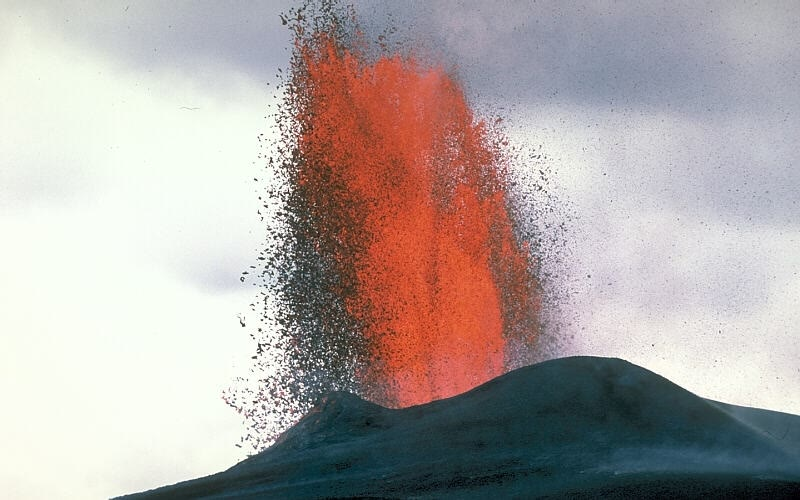
\includegraphics[height=4.3cm]{images/book4/b2-kilauea-fountain.jpg}\hfill
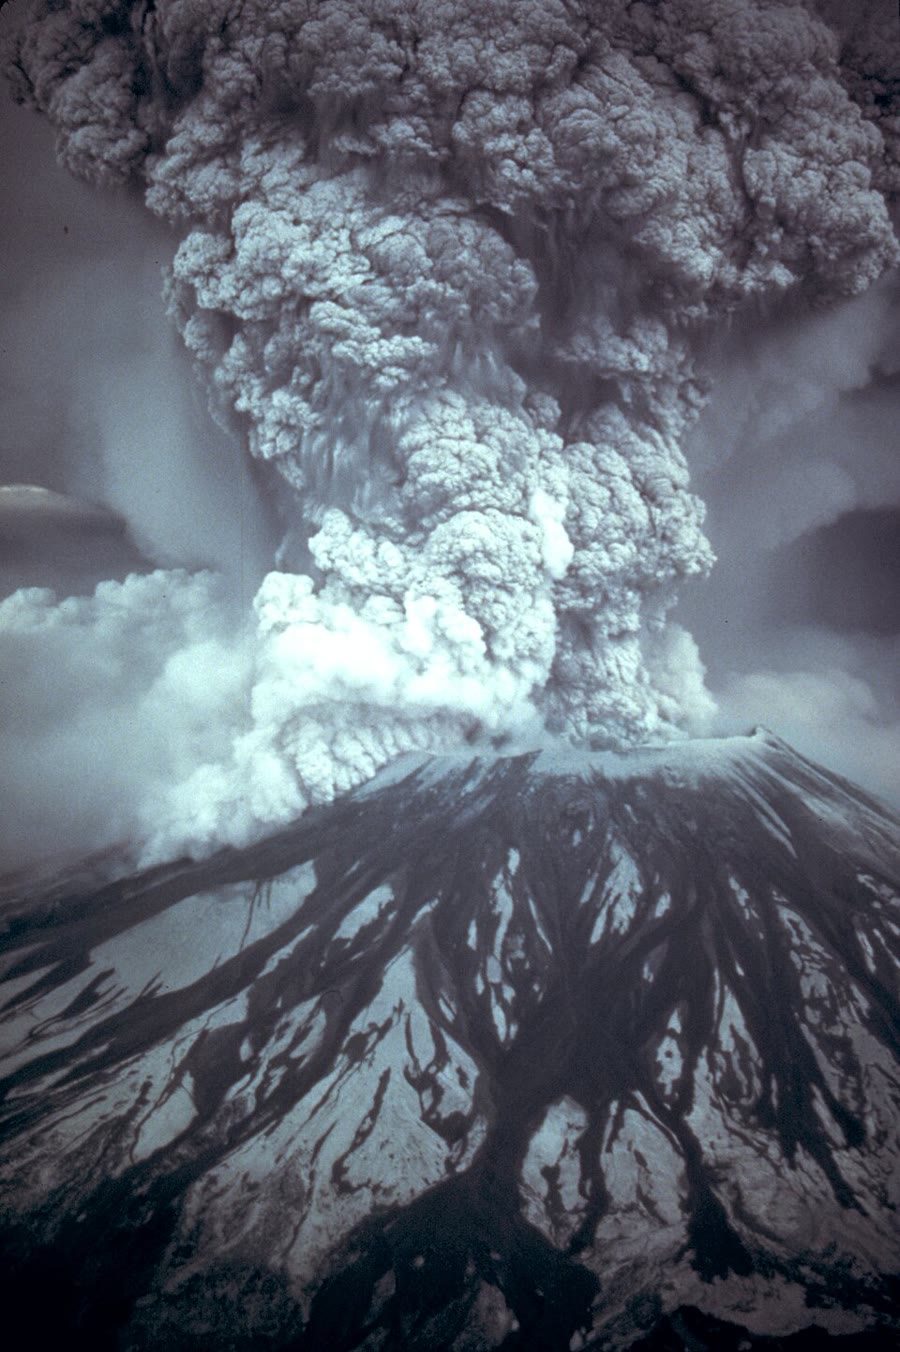
\includegraphics[height=4.3cm]{images/book4/b2-st-helens-column.jpg}\hfill
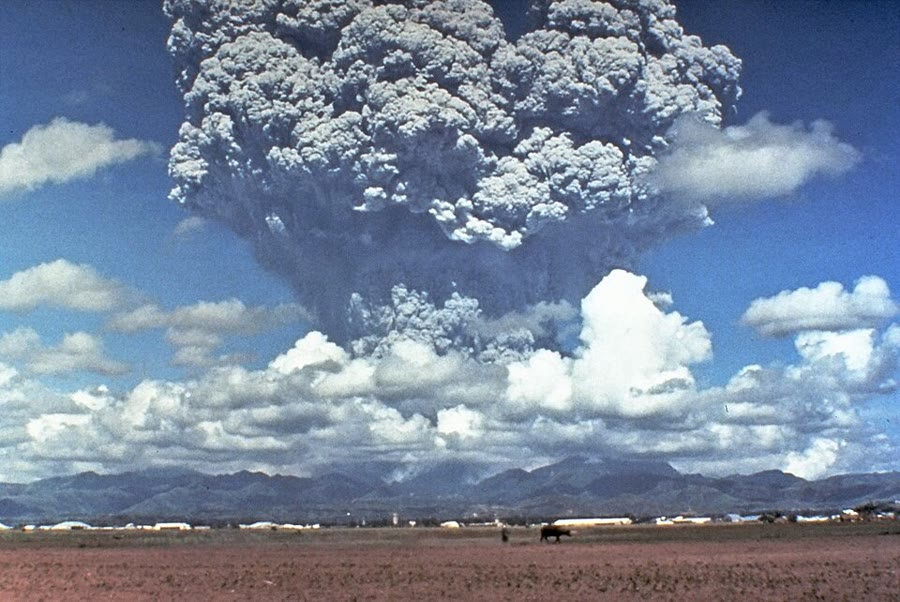
\includegraphics[height=4.3cm]{images/book4/b2-pinatubo-column.jpg}
\par\smallskip{\small اليمين: نافورة هاوايية على مخروط بوؤو أوؤو في كيلاويا،
أكتوبر 1983 \babelsublr{(J.\,D.~Griggs, USGS)}. الوسط: العمود البليني لجبل سانت هيلينز،
18 مايو 1980 \babelsublr{(Austin Post, USGS)}. اليسار: \omterm{def:b2:eruptive-styles:column}{عمود ثوران} جبل بيناتوبو في
12 يونيو 1991، قبل ثلاثة أيام من الثوران الذروي \babelsublr{(Dave Harlow, USGS)}. والصور
الثلاث كلها في الملك العام.}
\end{omfigure}
% ledger: usgs:puuoo, usgs:msh-may18, usgs:pinatubo-1991

\section{أعمدة الثوران}

\begin{definition}[عمود الثوران]\label{def:b2:eruptive-styles:column}
\emph{عمود الثوران}\index{عمود الثوران} هو الكتلة الصاعدة من الغاز
والقطع فوق منفذ انفجاري. وله ثلاثة أجزاء: \emph{النفّاث}، أو
منطقة الدفع الغازي، حيث يغادر المزيج المنفذ بسرعة لكنه أكثف من
الهواء ويصعد بزخمه؛ ومنطقة \emph{الحمل}، حيث يصعد المزيج،
بعد أن ابتلع من الهواء وسخّن ما يكفي ليصير أخفّ مما حوله،
بالطفو؛ و\emph{السحابة المظلّية}، التي تنتشر جانبيًا عند
المستوى الذي تساوي فيه كثافة العمود كثافة الغلاف الجوي.
\end{definition}
% ledger: usgs:glossary-ch6, nps:styles, aubry23:fits

\begin{omfigure}
\centering
\begin{tikzpicture}[x=1cm, y=1cm, font=\scriptsize]
% atmosphere and ground
\fill[blue!6] (-6.2,0) rectangle (6.2,6.4);
% volcano
\fill[brown!45, draw=brown!70!black] (-4.8,0) -- (-0.45,1.6) -- (0.45,1.6) -- (4.8,0) -- cycle;
% collapse branch (left): a density current hugging the flank
\fill[gray!55] (-0.45,1.6) -- (-0.7,2.35) .. controls (-1.1,2.25) and (-1.5,1.65) .. (-2.2,1.3)
  .. controls (-3.4,0.85) and (-4.6,0.42) .. (-5.9,0.28) -- (-5.9,0) -- (-4.8,0) -- cycle;
% jet
\fill[gray!70] (-0.45,1.6) -- (0.45,1.6) -- (0.75,2.5) -- (-0.75,2.5) -- cycle;
% convective column
\fill[gray!45] (-0.75,2.5) .. controls (-1.1,3.2) and (-1.0,3.8) .. (-1.4,4.2)
  -- (1.4,4.2) .. controls (1.0,3.8) and (1.1,3.2) .. (0.75,2.5) -- cycle;
% umbrella
\fill[gray!35] (-1.4,4.2) .. controls (-3,4.1) and (-5,4.2) .. (-5.8,4.45)
  .. controls (-5,4.9) and (-3,5.1) .. (0,5.25) .. controls (3,5.1) and (5,4.9) .. (5.8,4.45)
  .. controls (5,4.2) and (3,4.1) .. (1.4,4.2) -- cycle;
\draw[densely dashed, blue!60!black] (-6.2,4.4) -- (6.2,4.4);
% fallout from the far end of the umbrella, down to the ground
\foreach \x in {4.95,5.25,5.55} {\draw[gray!70, densely dotted, thick] (\x,4.3) -- (\x-0.1,0.02);}
\draw[gray, densely dotted] (0.45,1.6) -- (6.0,1.6);
\draw[<->] (6.0,1.6) -- (6.0,5.25) node[midway, right, align=left] {ارتفاع\\القمّة\\$H$\\فوق\\المنفذ};
% labels
\node[anchor=north west, align=left, blue!60!black] at (-6.1,4.3) {مستوى الطفو\\\foreignlanguage{arabic}{المتعادل (متقطّع)}};
\draw (-0.95,3.3) -- (-1.8,3.05) node[left, align=right] {منطقة الحمل:\\طافية، تسحب الهواء};
\draw (0.3,2.05) -- (2.0,2.35) node[right, align=left] {النفّاث: بالزخم،\\أكثف من الهواء};
\draw (2.6,4.85) -- (3.2,5.75) node[right] {السحابة المظلّية};
\node[anchor=east, align=right] at (4.8,1.25) {تساقط من\\السحابة المظلّية};
\draw (-3.4,0.7) -- (-3.9,1.5) node[above, align=center] {انهيار: تيار فتاتي\\بركاني كثيف};
\draw[-latex] (0,1.0) -- (0,1.55);
\node[anchor=north] at (0,1.0) {المنفذ};
\end{tikzpicture}
\par\smallskip{\small تشريح \omterm{def:b2:eruptive-styles:column}{عمود ثوران} (تخطيطي، بلا مقياس). على
اليمين يصعد العمود عبر مناطقه الثلاث وتُسقط السحابة المظلّية
\omterm{def:b2:eruptive-styles:tephra}{التيفرا} وهي تنتشر؛ وعلى اليسار أخفق جزء من النفّاث في أن يصير
طافيًا فانهار في تيار فتاتي بركاني كثيف.}
\end{omfigure}

يتوقف ارتفاع العمود قبل كل شيء على كمية الحرارة التي يجلبها في كل
ثانية، أي على معدل الثوران الكتلي~$Q$. ويعطي التحليل البعدي
شكل القانون.

\begin{proposition}[ارتفاع عمود طافٍ]\label{prop:b2:eruptive-styles:plume}
إذا كان ارتفاع القمّة $H$ لعمود طافٍ فوق مصدر نقطي مستقر لا يتوقف إلا
على دفق الطفو للمصدر $F$ (بُعده $\mathrm{m^4\,s^{-3}}$) وعلى
تردّد الطفو $N$ لغلاف جوي مستقر التطبّق (بُعده
$\mathrm{s^{-1}}$)، فإن
\[
H = c\,F^{1/4}N^{-3/4}
\]
حيث $c$ ثابت لا بُعدي. وبما أن $F$ يتناسب مع الدفق الحراري، ومن ثمّ
مع معدل الثوران الكتلي، فإن $H \propto Q^{1/4}$ في غلاف جوي معطى.
\end{proposition}

\begin{proof}
لنكتب $H = c\,F^{\alpha}N^{\beta}$. مطابقة الأطوال تعطي $4\alpha = 1$؛ ومطابقة
الأزمنة تعطي $-3\alpha - \beta = 0$. ومنه $\alpha = 1/4$ و$\beta = -3/4$، ولا
توجد تركيبة أخرى من $F$ و$N$ لها بُعد الطول.
\end{proof}

يأتي الثابت $c$ من سرعة ابتلاع العمود للهواء، التي تعالجها نظرية الأعمدة
بمعامل سحب مقيس في التجارب؛ ونقبله
هنا. والأعمدة الحقيقية ليست مصادر نقطية مستقرة في غلاف جوي ساكن، ولذلك
يضبط علماء البراكين القانون على ثورانات قيس فيها الارتفاع ومعدل الثوران الكتلي
كلاهما.
% ledger: aubry23:fits

\begin{proposition}[ارتفاع العمود ومعدل الثوران الكتلي]\label{prop:b2:eruptive-styles:mastin}
من أجل ارتفاع القمّة $H$ فوق المنفذ بالكيلومتر ومعدل الثوران الكتلي
$Q$ بالكيلوغرام في الثانية، تعطي مجموعة الثورانات الموثّقة جيدًا
\[
H = 0.304\,Q^{0.241},
\]
وتعطي مجموعة بيانات مستقلة أكبر من 130 حدثًا $H = 0.345\,Q^{0.226}$.
والتشتّت كبير: فالخطأ النسبي الجذري التربيعي المتوسط على $H$ هو
\qtyrange{53}{60}{\percent}.
\end{proposition}
\admitted
% ledger: aubry23:fits

كلا الأسّين قريب من $1/4$ في نظرية الأعمدة. ويبيّن الشكل أدناه
الضبطين والثورانات المثالية التي تستند إليها معاملات المصدر التي تستعملها
مراكز التنبّؤ بالرماد. فعمود ارتفاعه \qty{15}{km}، كعمود جبل
سانت هيلينز، يحتاج إلى \qty{e7}{kg/s}، أي عشرة آلاف طن في كل ثانية؛ ومضاعفة
الارتفاع تحتاج إلى نحو ثمانية عشر ضعف المعدل. وبالقراءة في الاتجاه المعاكس، يعطي الارتفاع المقيس
المعدل، لكن في حدود عامل من عدّة أضعاف فقط، لأن $Q$ يتناسب مع $H^4$
(\cref{exo:b2:eruptive-styles:3}). ويعبّر علماء البراكين عن المعدل ب\emph{الشدّة} $I =
\log_{10}Q + 3$، حيث $Q$ بالكيلوغرام في الثانية.
% ledger: mastin09:examples, aubry23:fits, brown14:record

\begin{omfigure}
\centering
\begin{tikzpicture}
\begin{axis}[omrecord, width=0.82\linewidth, height=6cm, xmode=log, ymode=log,
  xmin=1e3, xmax=1e9, ymin=1, ymax=60,
  xlabel={\foreignlanguage{arabic}{معدل الثوران الكتلي $Q$ \babelsublr{(\unit{kg/s})}}}, ylabel={\foreignlanguage{arabic}{ارتفاع القمّة فوق المنفذ \babelsublr{(\unit{km})}}},
  ytick={1,2,5,10,20,50}, yticklabels={1,2,5,10,20,50},
  legend pos=north west, legend style={font=\scriptsize},
  tick label style={font=\scriptsize}, label style={font=\small}]
\addplot[very thick, black] table[x=Q, y=mastin] {figdata/out/bachelor-2-eruptions-column.dat};
\addlegendentry{$H = 0.304\,Q^{0.241}$}
\addplot[thick, red!70!black, dashed] table[x=Q, y=aubry] {figdata/out/bachelor-2-eruptions-column.dat};
\addlegendentry{$H = 0.345\,Q^{0.226}$}
\addplot[only marks, mark=*, mark size=1.8pt, blue!70!black]
  table[x=Q, y=H] {figdata/out/bachelor-2-eruptions-column-data.dat};
\addlegendentry{ثورانات مثالية}
\begin{scope}[font=\tiny, inner sep=1.5pt]
\node[anchor=north west] at (axis cs:5e3,2) {\foreignlanguage{arabic}{إتنا 2001}};
\node[anchor=south east] at (axis cs:1e5,7) {\foreignlanguage{arabic}{سيرو نيغرو 1992}};
\node[anchor=north west] at (axis cs:2e5,5) {\foreignlanguage{arabic}{روابيهو 1996}};
\node[anchor=east] at (axis cs:1e6,10) {\foreignlanguage{arabic}{فويغو 1974}};
\draw[gray] (axis cs:3e6,10) -- (axis cs:2e7,4.5) node[anchor=west, black] {تلال سوفرير};
\draw[gray] (axis cs:4e6,11) -- (axis cs:2e7,6.5) node[anchor=west, black] {\foreignlanguage{arabic}{سبير 1992}};
\node[anchor=south east] at (axis cs:1e7,15) {\foreignlanguage{arabic}{سانت هيلينز 1980}};
\node[anchor=south east, align=right] at (axis cs:1e8,25) {سانت هيلينز\\سحابة الإغنمبريت};
\end{scope}
\end{axis}
\end{tikzpicture}
\par\smallskip{\small ارتفاع قمّة \omterm{def:b2:eruptive-styles:column}{أعمدة الثوران} فوق المنفذ بدلالة
معدل الثوران الكتلي: الضبط التجريبي لماستن وآخرين (2009)، وضبط
أوبري وآخرين (2023) على مجموعة بيانات مستقلة، والثورانات المثالية
في المجموعة الأولى (صعدت سحابة \omterm{def:b2:eruptive-styles:pdc}{الإغنمبريت} لجبل سانت هيلينز من
التدفّقات الفتاتية البركانية، لا من المنفذ).}
\end{omfigure}
% ledger: aubry23:fits, mastin09:examples

وقد يُخفق العمود أيضًا في الصعود. فالنفّاث يغادر المنفذ أكثف من الهواء؛ فإن
نفد زخمه قبل أن يبتلع من الهواء ما يكفي ليصير طافيًا،
لانخفاض محتواه الغازي مثلًا، ينهار العمود ويندفع المزيج
على الأجناب تيارًا ساخنًا كثيفًا. ويمكن للأعمدة البلينية أن تنهار على
هذا النحو، وفي بيناتوبو ملأت التدفّقات الفتاتية البركانية لعام 1991 الأودية
برواسب يصل سمكها إلى \qty{200}{m}.
% ledger: nps:styles, usgs:pinatubo-deposits

\section{النواتج الفتاتية البركانية}

\begin{definition}[التيفرا والقطع الفتاتية البركانية]\label{def:b2:eruptive-styles:tephra}
\emph{القطعة الفتاتية البركانية}\index{القطعة الفتاتية البركانية} قطعة ينتجها التفتّت
الانفجاري للصهارة أو للصخور المحيطة بها. و\emph{التيفرا}\index{التيفرا}
الاسم الجامع لكل القطع الفتاتية البركانية المقذوفة في الهواء، أيًّا كان حجمها.
فحسب الحجم، تكوّن القطع الأدقّ من \qty{2}{mm} الرماد البركاني؛ والتي
من \qtyrange{2}{64}{mm} هي \emph{اللابيلي}\index{اللابيلي}؛ والأكبر من
\qty{64}{mm} كتل إن كانت صلبة حين قُذفت وزاويّة،
و\emph{قنبلة بركانية}\index{القنبلة البركانية} إن كانت منصهرة كليًا أو جزئيًا
واتّخذت في الطيران شكلًا مستديرًا أو مغزليًا.
\end{definition}
% ledger: nps:pyroclast-sizes, usgs:glossary-ch6

تسقط \omterm{def:b2:eruptive-styles:tephra}{التيفرا} من السحابة المظلّية ومن العمود مع اتجاه الريح راسبًا متساقطًا
يغطّي الأرض: ثخينًا قرب المنفذ، وأرقّ وأنعم بعيدًا عنه. ويُرسم
سمكه ب\emph{خطوط تساوي السمك}، وهي خطوط السمك المتساوي، وهو، كقاعدة عامة،
يتناقص أسّيًا مع المسافة. ولأن الريح تمطّ خطوط تساوي السمك
إلى قطوع ناقصة، فإن أفضل قياس للمسافة هو الجذر التربيعي للمساحة التي يحيط بها
كل خط تساوي سمك.
% ledger: usgs:ash-props, biass19:layer5

\begin{proposition}[حجم راسب يرقّ أسّيًا]\label{prop:b2:eruptive-styles:thinning}
إذا تناقص سمك راسب متساقط مع الجذر التربيعي $x = \sqrt A$
لمساحة خط تساوي السمك وفق $T = T_0\,e^{-kx}$، فإن حجمه الكلي هو
\[
V = \frac{2T_0}{k^2}.
\]
ويقع نصف هذا الحجم خارج خط تساوي السمك $x_{1/2} = 1.678/k$.
\end{proposition}

\begin{proof}
بين خطّي تساوي السمك اللذين مساحتاهما $A$ و$A + dA$ يكون حجم الراسب $T\,dA$،
و$dA = 2x\,dx$. ومنه $V = \int_0^\infty T_0e^{-kx}\,2x\,dx = 2T_0/k^2$،
بالتكامل بالتجزئة ($\int_0^\infty xe^{-kx}dx = 1/k^2$). والحجم داخل $x$
هو $\frac{2T_0}{k^2}[1 - (1 + kx)e^{-kx}]$، وهو نصف الحجم الكلي حين $(1 +
u)e^{-u} = 1/2$ مع $u = kx$، أي $u = 1.678$.
\end{proof}

الرواسب الحقيقية ترقّ بميلين أو أكثر، شديد قرب المنفذ ولطيف
بعيدًا عنه، لأن \omterm{def:b2:eruptive-styles:tephra}{اللابيلي} الخشنة تسقط بسرعة من العمود والرماد الناعم
ينجرف. ويُضبط كل مقطع على حدة ويؤخذ التكامل مقطعًا
مقطعًا.

\begin{method}[حجم راسب متساقط من خطوط تساوي سمكه]\label{met:b2:eruptive-styles:volume}
ارسم $\ln T$ بدلالة $\sqrt A$ لكل خط تساوي سمك واضبط مستقيمًا على كل
سلسلة من النقاط المصطفّة. ومن أجل مقطعين، $T_0e^{-k_1x}$ داخل نقطة التقاطع
$X$ للمستقيمين والثاني خارجها، يكون الحجم
\[
V = \frac{2T_0}{k_1^2} + 2T_0e^{-k_1X}\left[\frac{k_2X + 1}{k_2^2} -
\frac{k_1X + 1}{k_1^2}\right]
\]
(\cref{exo:b2:eruptive-styles:10}). وحوّل الحجم الكلي إلى مكافئ الصخر الكثيف، أي حجم
الكتلة نفسها صهارةً خالية من الفقاعات، بالعلاقة $V_{\mathrm{DRE}} = V\rho_{\mathrm{deposit}}/\rho_{\mathrm{magma}}$.
\end{method}
% ledger: biass19:layer5, brown14:record

يطبّق الشكل أدناه الطريقة على راسب خبث بركاني متساقط قذفه كوتوباكسي، في
الإكوادور، قبل نحو \num{1200} سنة. يضبط مقطعان خطوط تساوي السمك الستة،
بمسافتَي تنصيف للسمك $\ln 2/k$ قدرهما \qty{1.9}{km} و\qty{5.0}{km} (وتجد
الدراسة المنشورة، التي يختلف ضبطها قليلًا، \qty{1.9}{km}
و\qty{5.3}{km})، ويخرج الحجم \qty{0.29}{km^3}، كما في تلك الدراسة. وأكثر من
\qty{40}{\percent} منه يقع في المقطع البعيد الرقيق، ولهذا يهمّ الرماد البعيد،
السهل الحتّ أو الذي لم يُرسم قطّ، إلى هذا الحدّ في الحجم الكلي. وللرماد المتساقط حديثًا
كثافة كلية من \qtyrange{500}{1500}{kg/m^3}، أدنى بكثير من كثافة
\omterm{def:b2:magma-emplacement:magma}{الصهارة}، فيكون مكافئ الصخر الكثيف نحو نصف الحجم الكلي أو أقل.
% ledger: biass19:layer5, usgs:ash-props

\begin{omfigure}
\centering
\begin{tikzpicture}
\begin{axis}[omrecord, width=0.78\linewidth, height=5.6cm, ymode=log,
  xmin=0, xmax=30, ymin=2, ymax=2000,
  xlabel={\foreignlanguage{arabic}{$\sqrt{\text{مساحة خط تساوي السمك}}$ \babelsublr{(\unit{km})}}}, ylabel={\foreignlanguage{arabic}{السمك \babelsublr{(\unit{cm})}}},
  ytick={2,5,10,20,50,100,200,500,1000,2000}, yticklabels={2,5,10,20,50,100,200,500,1000,2000},
  legend pos=north east, legend style={font=\scriptsize},
  tick label style={font=\scriptsize}, label style={font=\small}]
\addplot[thick, black, restrict x to domain=0:12] table[x=sqrtA_km, y=seg1] {figdata/out/bachelor-2-eruptions-thin-fit.dat};
\addlegendentry{\foreignlanguage{arabic}{المقطع القريب، $k_1 = \qty{0.365}{km^{-1}}$}}
\addplot[thick, red!70!black, dashed, restrict x to domain=5:30] table[x=sqrtA_km, y=seg2] {figdata/out/bachelor-2-eruptions-thin-fit.dat};
\addlegendentry{\foreignlanguage{arabic}{المقطع البعيد، $k_2 = \qty{0.138}{km^{-1}}$}}
\addplot[only marks, mark=*, mark size=2pt, blue!70!black] table[x=sqrtA_km, y=T_cm] {figdata/out/bachelor-2-eruptions-thin-data.dat};
\addlegendentry{خطوط تساوي السمك}
\end{axis}
\end{tikzpicture}
\par\smallskip{\small ترقّق راسب الخبث البركاني المتساقط في الطبقة~5 من كوتوباكسي (الإكوادور)،
الذي يبلغ عمره نحو \num{1200} سنة: سمك خطوط تساوي السمك عند بياس وبونادونا
وهوتون (2019) بدلالة الجذر التربيعي للمساحة التي يحيط بها كل خط (والسلّم
الرأسي لوغاريتمي). ويتقاطع مقطعان أسّيان، مضبوطان على خطّي تساوي السمك
القريبين وعلى الخطوط الأربعة البعيدة، عند $\sqrt A = \qty{8.6}{km}$؛
وبالتكامل يعطيان حجمًا كليًا قدره \qty{0.29}{km^3}.}
\end{omfigure}
% ledger: biass19:layer5

ليست كل \omterm{def:b2:eruptive-styles:tephra}{التيفرا} تسقط من السماء. فحين ينهار عمود، أو تتفتّت قبّة، أو
يمزّق انفجار جانبي جانب البركان، يجري المزيج الساخن على
الأرض.

\begin{definition}[التيارات الفتاتية البركانية الكثيفة]\label{def:b2:eruptive-styles:pdc}
\emph{التيار الفتاتي البركاني الكثيف}\index{التيار الفتاتي البركاني الكثيف} مزيج من
غاز ساخن وقطع فتاتية بركانية يلتصق بالأرض ويجري نحو الأسفل أو إلى الخارج
لأنه أكثف من الهواء. و\emph{التدفّق الفتاتي البركاني}\index{التدفّق الفتاتي البركاني}
تيار مركّز من قطع الصخر والرماد والغاز، درجة حرارته عمومًا
\qtyrange{200}{700}{\celsius}، يتحرك بعشرات الأمتار في الثانية؛
و\emph{الموجة الفتاتية البركانية}\index{الموجة الفتاتية البركانية} سحابة أكثر تخفيفًا من الرماد
والصخر والغاز، درجة حرارتها عدّة مئات من الدرجات، تتحرك بسرعة رياح
الإعصار. و\emph{الإغنمبريت}\index{الإغنمبريت} هو الصخر الذي ترسّبه التيارات
الفتاتية البركانية الكثيفة، وقد يلتحم بحرارته الذاتية.
\end{definition}
% ledger: usgs:glossary-ch6

في 18 مايو 1980 كشف انهيار الجناح الشمالي لجبل سانت هيلينز، وهو أكبر
انزلاق أرضي في التاريخ المسجّل بنحو \qty{2.8}{km^3}، الصهارةَ
وأطلق انفجارًا جانبيًا اجتاح نحو \qty{600}{km^2} بسرعة تصل إلى
\qty{480}{km/h}؛ ثم بلغت تدفّقات فتاتية بركانية لا تقل حرارتها عن \qty{700}{\celsius}
مسافة \qty{8}{km} من الفوّهة. وكانت تدفّقات بيناتوبو لعام 1991 لا تزال ساخنة حتى
\qty{500}{\celsius} في داخلها بعد خمس سنوات.
% ledger: usgs:msh-may18, usgs:msh-flows, usgs:msh-reach, usgs:pinatubo-deposits

\begin{definition}[اللاهار]\label{def:b2:eruptive-styles:lahar}
\emph{اللاهار}\index{اللاهار} مزيج سريع الحركة من الماء والحطام البركاني
يجري في وادٍ نهري، بقوام يتراوح بين الماء الموحل
والخرسانة الرطبة. وتتكوّن اللاهارات حين تذيب التيارات الفتاتية البركانية الثلج والجليد، أو حين
تسقط أمطار غزيرة على رواسب بركانية مفكّكة، أو حين تنفجر بحيرة حجزتها رواسب
بركانية، أو من انهيار ركامي.
\end{definition}
% ledger: usgs:glossary-ch6

\omterm{def:b2:eruptive-styles:lahar}{اللاهارات} تعيش أطول من الثورانات. فحول بيناتوبو حوّلت أمطار الرياح الموسمية والأعاصير
رماد عام 1991 إلى \omterm{def:b2:eruptive-styles:lahar}{لاهارات} طوال سنوات، وتسبّبت في دمار أكبر مما سبّبه
الثوران نفسه.
% ledger: usgs:pinatubo-lahars

\begin{definition}[الكالديرا]\label{def:b2:eruptive-styles:caldera}
\emph{الكالديرا}\index{الكالديرا} منخفض بركاني كبير على شكل حوض،
عرضه \qtyrange{2}{50}{km} وأوسع بكثير من أي منفذ داخله، تكوّن
بانهيار الأرض في خزّان صهاري ضحل أفرغه ثوران
جزئيًا.
\end{definition}
% ledger: usgs:glossary-ch6

كالديرا بيناتوبو وكالديرا نوفاروبتا عرض كلٍّ منهما نحو \qty{2.5}{km}، عند
الطرف الصغير من المدى. وتختلف \omterm{def:b2:eruptive-styles:caldera}{الكالديرا} عن الفوّهة، وهي أصغر وتحفرها الانفجارات.
% ledger: usgs:pinatubo-1991, nps:styles, usgs:glossary-ch6

\section{قياس الثورانات وعدّها}

\begin{definition}[مؤشر الانفجارية البركانية]\label{def:b2:eruptive-styles:vei}
\emph{مؤشر الانفجارية البركانية}\index{مؤشر الانفجارية البركانية} (VEI)
عدد صحيح من 0 إلى 8 يقيس حجم الثوران، أساسًا بالحجم
الكلي لتيفراه: VEI~0 لأقل من \qty{e4}{m^3}، وVEI~1 حتى
\qty{e6}{m^3}، ثم درجة واحدة لكل عامل عشرة، حتى VEI~8 فوق
\qty{e12}{m^3}، أي \qty{1000}{km^3}. ويُستعمل ارتفاع العمود وأوصاف الثوران
حين لا يكون الحجم معروفًا. والثوران غير الانفجاري مؤشره VEI~0،
أيًّا كان حجم حممه.
\end{definition}
% ledger: usgs:vei-criteria, usgs:msh-comparisons

\begin{table}[ht]
\centering
\small
\begin{tabular}{llll}
\hline
VEI & حجم \omterm{def:b2:eruptive-styles:tephra}{التيفرا} الكلي (\unit{m^3}) & ارتفاع العمود (\unit{km}) & الطراز المعتاد \\
\hline
0 & $< 10^{4}$ & $< 0.1$ & هاوايي \\
1 & \mbox{\textdir TLT $10^{4}$--$10^{6}$} & \mbox{\textdir TLT 0.1--1} & هاوايي، سترومبولي \\
2 & \mbox{\textdir TLT $10^{6}$--$10^{7}$} & \mbox{\textdir TLT 1--5} & سترومبولي، فولكاني \\
3 & \mbox{\textdir TLT $10^{7}$--$10^{8}$} & \mbox{\textdir TLT 3--15} & فولكاني \\
4 & \mbox{\textdir TLT $10^{8}$--$10^{9}$} & \mbox{\textdir TLT 10--25} & فولكاني، بليني \\
5 & \mbox{\textdir TLT $10^{9}$--$10^{10}$} & $> 25$ & بليني \\
6 & \mbox{\textdir TLT $10^{10}$--$10^{11}$} & $> 25$ & بليني \\
7 & \mbox{\textdir TLT $10^{11}$--$10^{12}$} & $> 25$ & بليني \\
8 & $> 10^{12}$ & $> 25$ & بليني \\
\hline
\end{tabular}
\caption{معايير \omterm{def:b2:eruptive-styles:vei}{مؤشر الانفجارية البركانية} (عن نيوهول وسيلف، 1982).}
\label{tab:b2:eruptive-styles:vei}
\end{table}
% ledger: usgs:vei-criteria

المؤشر لوغاريتمي كمقدار الزلزال، لكنه أخشن. فجبل
سانت هيلينز في 1980، بما قذفه من \qty{1.3}{km^3} من الرماد، صُنّف VEI~5 «بالكاد»؛
وصُنّف بيناتوبو في 1991 VEI~6؛ وتامبورا في 1815، الذي قذف من الرماد ما بين ثلاثين وثمانين
ضعف ما قذفه جبل سانت هيلينز، صُنّف VEI~7، أكبر \omterm{def:b2:eruptive-styles:regimes}{ثوران انفجاري}
في التاريخ المدوّن. وفي العمل الكمّي يفضّل علماء البراكين
\emph{المقدار} $M = \log_{10}m - 7$، حيث $m$ الكتلة المقذوفة بالكيلوغرام، الذي
يتجنّب الكثافة الكلية للراسب، والشدّة المعرّفة أعلاه من أجل
المعدل.
% ledger: usgs:msh-1980-ash, usgs:msh-comparisons, data:b4-gvp-eruptions, brown14:record

الثورانات الصغيرة متكرّرة والكبيرة نادرة. ويجعل الفهرس العالمي
لثورانات الهولوسين العلاقة كمّية، بشرط أن تُراعى
ثغراته: فالثوران لا يدخل الفهرس إلا إن سجّله أحد أو عُثر على
راسبه، والثورانات الصغيرة البعيدة عن المراقبين، أو التي يزيد عمرها على بضعة قرون،
كثيرًا ما فاتت. وسجلّ الثورانات الكبيرة مكتمل على مدى أطول من
سجلّ الصغيرة. وفي اللوحة اليسرى من الشكل أدناه تتراكم ثورانات كل
حجم المسجّلة منذ 1500 مع الزمن؛ ولو كان السجلّ مكتملًا بمعدل ثابت
لاتّبع القطر. وثورانات VEI~3 أو أكثر تتكدّس في القرن
الأخير، لأن معظم الأقدم منها لم يُسجَّل قطّ؛ أمّا سجلّ VEI~6
فقريب من القطر.
% ledger: data:b4-gvp-eruptions, brown14:record

\begin{dated}{2026}
يُدرج فهرس برنامج البراكين العالمي \num{7747} ثورانًا هولوسينيًا مؤكّدًا
ذا مؤشر VEI. وبالعدّ من بداية نافذة إلى نهاية 2024، كان هناك
399 ثورانًا من VEI~3 أو أكثر منذ 1950، و95 من VEI~4 أو أكثر منذ 1900،
و22 من VEI~5 أو أكثر منذ 1800، و8 من VEI~6 أو أكثر منذ 1500 (وأحدثها
بيناتوبو في 1991). ولم يُسجَّل إلا ثورانان من VEI~7 منذ العام
1000: رينجاني في 1257 وتامبورا، الذي بدأ ثورانه في 1812 وبلغ ذروته في
1815.
\end{dated}
% ledger: data:b4-gvp-eruptions, usgs:msh-comparisons

\begin{proposition}[قانون التكرار والحجم للثورانات]\label{prop:b2:eruptive-styles:frequency}
ليكن $\lambda_v$ متوسط عدد الثورانات ذات \mbox{\textdir TLT VEI $\ge v$} في السنة على الأرض،
وكلٌّ منها مقدّر على نافذة يكون فيها سجلّه قريبًا من الاكتمال (من 1950
من أجل $v = 3$، و1900 من أجل $v = 4$، و1800 من أجل $v = 5$، و1500 من أجل $v = 6$). عندئذ، بالمربعات
الصغرى،
\[
\log_{10}\lambda_v = 3.28 - 0.85\,v .
\]
وكل درجة من VEI أندر بنحو سبع مرات من الدرجة التي تحتها.
\end{proposition}
% ledger: data:b4-gvp-eruptions

القانون تجريبي، ضبط على أربع نقاط، ويتوقف أسّه على
النوافذ المختارة؛ وهو يتنبّأ بثوران واحد من VEI~7 أو أكثر كل \num{470} سنة،
قريبًا من الثورانين في الألف سنة الأخيرة اللذين لم يُستعملا في ضبطه. وبما أن
الثورانات مستقلة بعضها عن بعض تقريبًا، فهي تسلك سلوك عملية
بواسون، ويكون احتمال ثوران واحد على الأقل ذي \mbox{\textdir TLT VEI $\ge v$} في $t$ سنة
هو $1 - e^{-\lambda_vt}$ (مسألة نهاية الأسبوع).
% ledger: data:b4-gvp-eruptions

\begin{omfigure}
\centering
\begin{tikzpicture}
\begin{axis}[omrecord, name=cum, width=0.47\linewidth, height=5.6cm,
  xmin=1500, xmax=2024, ymin=0, ymax=1,
  xlabel={السنة}, ylabel={الحصّة المسجّلة منذ 1500},
  xtick={1500,1600,1700,1800,1900,2000}, x tick label style={/pgf/number format/1000 sep={}},
  legend pos=north west, legend style={font=\tiny},
  tick label style={font=\scriptsize}, label style={font=\small}]
\addplot[thick, gray, densely dotted, domain=1500:2024, samples=2] {(x - 1500)/524};
\addlegendentry{معدل ثابت}
\addplot[thick, blue!70!black] table[x=year, y=f3] {figdata/out/bachelor-2-eruptions-vei-cumul.dat};
\addlegendentry{VEI $\ge 3$}
\addplot[thick, black, dashed] table[x=year, y=f4] {figdata/out/bachelor-2-eruptions-vei-cumul.dat};
\addlegendentry{VEI $\ge 4$}
\addplot[thick, orange!80!black, dashdotted] table[x=year, y=f5] {figdata/out/bachelor-2-eruptions-vei-cumul.dat};
\addlegendentry{VEI $\ge 5$}
\addplot[thick, red!70!black, const plot] table[x=year, y=f6] {figdata/out/bachelor-2-eruptions-vei-cumul.dat};
\addlegendentry{VEI $\ge 6$}
\end{axis}
\begin{axis}[omrecord, at={(cum.east)}, anchor=west, xshift=1.9cm,
  width=0.47\linewidth, height=5.6cm, ymode=log,
  xmin=2.5, xmax=7.5, ymin=1e-3, ymax=20,
  xlabel={المؤشر \babelsublr{VEI $v$}}, ylabel={الثورانات ذات \babelsublr{VEI $\ge v$} في السنة},
  xtick={3,4,5,6,7},
  tick label style={font=\scriptsize}, label style={font=\small}]
\addplot[thick, black] table[x=vei, y=rate] {figdata/out/bachelor-2-eruptions-vei-fit.dat};
\addplot[only marks, mark=*, mark size=2pt, blue!70!black] table[x=vei, y=rate] {figdata/out/bachelor-2-eruptions-vei-rate.dat};
\addplot[only marks, mark=o, mark size=2.4pt, red!70!black] table[x=vei, y=rate] {figdata/out/bachelor-2-eruptions-vei-rate7.dat};
\node[font=\tiny, anchor=south west] at (axis cs:3.05,6) {منذ 1950};
\node[font=\tiny, anchor=south west] at (axis cs:4.05,0.8) {منذ 1900};
\node[font=\tiny, anchor=south west] at (axis cs:5.05,0.1) {منذ 1800};
\node[font=\tiny, anchor=south west] at (axis cs:6.05,0.016) {منذ 1500};
\node[font=\tiny, anchor=east, red!70!black] at (axis cs:6.85,0.00195) {منذ 1000};
\end{axis}
\end{tikzpicture}
\par\smallskip{\small اليسار: اكتمال السجلّ العالمي. لكل حجم،
حصّة الثورانات المسجّلة بين 1500 و2024 التي كانت قد
وقعت حتى سنة معطاة؛ ولو كان السجلّ مكتملًا بمعدل ثابت لاتّبع
القطر المنقّط. اليمين: المعدل السنوي لثورانات \mbox{\textdir TLT VEI $\ge v$}، كلٌّ منها معدود على
نافذته الخاصة، ومستقيم المربعات الصغرى في
\cref{prop:b2:eruptive-styles:frequency}؛ والدائرة المفرغة، \mbox{\textdir TLT VEI $\ge 7$} منذ العام
1000، لم تُستعمل في الضبط. البيانات: برنامج البراكين العالمي، قاعدة بيانات براكين
العالم.}
\end{omfigure}
% ledger: data:b4-gvp-eruptions

\section{مراقبة البراكين}

لا تبلغ \omterm{def:b2:magma-emplacement:magma}{الصهارة} السطح دون إنذار. فعليها أن تكسر الصخر لتفتح
طريقها، وهي ترفع الأرض كلما تراكمت، وتحرّر الغاز كلما انخفض الضغط
عليها، وتسخّن الأرض. ومراصد البراكين تراقب هذه الأربعة كلها.

\emph{النشاط الزلزالي.} \omterm{def:b2:magma-emplacement:magma}{الصهارة} المتحرّكة عبر القشرة تكسر الصخر وتطلق أسرابًا
من الزلازل الصغيرة. فقبل 18 مايو 1980 أنتج جبل سانت هيلينز أكثر من
\num{10000} منها في شهرين؛ وأنتج بيناتوبو آلافًا بين أبريل
ويونيو 1991، من صهارة تصعد من عمق يزيد على \qty{32}{km}. والمقادير
والعزوم الزلزالية في مجلد السنة الأولى تنطبق دون تغيير؛ والمختلف هو
المصادر، شقوق تنفتح وقنوات مملوءة بالموائع ترنّ، إلى جانب الصدوع.
% ledger: usgs:msh-lead-up, usgs:pinatubo-deposits

\emph{التشوّه.} الخزّان الذي يمتلئ ينتفخ ويرفع الأرض التي
فوقه. وتقيس التسوية ومقاييس الميل وتحديد المواقع بالأقمار الصناعية هذا الرفع؛ ويرسمه قياس التداخل الراداري من الأقمار الصناعية على
براكين كاملة، وهي تقنية يشرحها مجلد السنة الثالثة من هذه السلسلة. وأبسط
نموذج يعامل الخزّان كرةً صغيرة.

\begin{proposition}[مصدر موغي]\label{prop:b2:eruptive-styles:mogi}
مصدر كروي صغير على عمق $z_0$ في نصف فضاء مرن متجانس
نسبة بواسون فيه $\nu$، يتغيّر حجمه بمقدار $\Delta V$، وهو ما يسمّى
\emph{مصدر موغي}\index{مصدر موغي}، يرفع السطح على مسافة أفقية $r$
بمقدار
\[
u_z(r) = \frac{(1 - \nu)\,\Delta V}{\pi}\,\frac{z_0}{(r^2 + z_0^2)^{3/2}} .
\]
\end{proposition}
\admitted
% ledger: dmodels:mogi

يبلغ الرفع أقصاه فوق المصدر، $u_z(0) = (1 - \nu)\Delta V/(\pi z_0^2)$،
وينخفض إلى نصف ذلك عند $r = z_0\sqrt{2^{2/3} - 1} = 0.766\,z_0$: فعرض
الانتفاخ يعطي عمق المصدر، ثم يعطي ارتفاعه تغيّر
الحجم. ولأن $\Delta V$ وحده يدخل في الصيغة، لا يمكن فصل الضغط في الخزّان عن حجمه،
ولذلك فإن ما يذكره الجيوديسيون هو تغيّرات الحجم لا الضغوط.
والصيغة هي الحدّ الأول من حلّ مضبوط لكرة نصف قطرها
$a$؛ والتصحيح \qty{12}{\percent} حين $a = z_0/2$ و\qty{3}{\percent}
حين $a = z_0/3$.
% ledger: dmodels:mogi

\begin{omfigure}
\centering
\begin{tikzpicture}
\begin{axis}[omrecord, width=0.78\linewidth, height=5.2cm,
  xmin=-12, xmax=12, ymin=0, ymax=65,
  xlabel={\foreignlanguage{arabic}{المسافة الأفقية عن المصدر \babelsublr{(\unit{km})}}}, ylabel={\foreignlanguage{arabic}{الرفع \babelsublr{(\unit{mm})}}},
  legend pos=north east, legend style={font=\scriptsize},
  tick label style={font=\scriptsize}, label style={font=\small}]
\addplot[very thick, black] table[x=r_km, y=z2] {figdata/out/bachelor-2-eruptions-mogi.dat};
\addlegendentry{\foreignlanguage{arabic}{مصدر على عمق \qty{2}{km}}}
\addplot[very thick, red!70!black, dashed] table[x=r_km, y=z4] {figdata/out/bachelor-2-eruptions-mogi.dat};
\addlegendentry{\foreignlanguage{arabic}{مصدر على عمق \qty{4}{km}}}
\draw[<->, thin] (axis cs:-1.532,29.8) -- (axis cs:1.532,29.8) node[midway, below, font=\tiny] {$2\times 0.766\,z_0$};
\end{axis}
\end{tikzpicture}
\par\smallskip{\small رفع السطح فوق \omterm{prop:b2:eruptive-styles:mogi}{مصدر موغي} يزداد حجمه بمقدار
\qty{e6}{m^3} ($\nu = 0.25$)، على عمقين. فعلى عمق مضاعف يكون الانتفاخ أخفض بأربع
مرات وأعرض بمرتين؛ ويحدّد السهم العرض الكامل عند نصف الارتفاع
للانتفاخ الضحل.}
\end{omfigure}
% ledger: dmodels:mogi

\emph{الغاز والحرارة.} كلما صعدت \omterm{def:b2:magma-emplacement:magma}{الصهارة} ونزعت غازها، ازداد دفق ثاني أكسيد الكبريت عند
السطح، وهو يقاس من الأرض ومن الطائرات ومن
الأقمار الصناعية؛ وقد أطلق بيناتوبو آلاف الأطنان منه في الأسابيع التي سبقت ثورانه.
وتظهر حرارة \omterm{def:b2:magma-emplacement:magma}{الصهارة} الضحلة في الصور الحرارية للأرض وللمنفذ.
% ledger: usgs:pinatubo-deposits

من هذه البيانات يحدّد المرصد مستوى إنذار. ففي الولايات المتحدة يتكوّن
مستوى الإنذار البركاني الأرضي، المعمول به منذ 2006، من أربع درجات: عادي (NORMAL)،
وتنبيه (ADVISORY)، ومراقبة (WATCH)، وإنذار (WARNING)، ويحذّر رمز لوني موازٍ للطيران، من الأخضر (GREEN) إلى الأحمر (RED)،
الطائرات من الرماد. ولا توجد عتبات ثابتة: فكل تغيير يقرّره
علماء المرصد من مجمل بيانات المراقبة، وسلوك البركان في الماضي،
وما يُعرف عن العمليات الجارية. ويبقى التنبّؤ
احتماليًا: فمتى يبدأ الثوران وما حجمه أمران يصعب
توقّعهما. وفي بيناتوبو سمح تنبّؤ عام 1991 للسكان القاطنين قرب
البركان بالابتعاد في الوقت المناسب وأنقذ \num{5000} حياة على الأقل. أمّا كيف تدخل هذه التنبّؤات
في القرارات المتعلقة بالخطر والمخاطرة فموضعه \cref{ch:b2:geological-hazards}.
% ledger: hvo:alert-levels, usgs:pinatubo-1991

\begin{inthefield}[في مرصد بركاني]
\begin{minipage}[t]{0.6\linewidth}\vspace{0pt}
يراقب المرصد براكينه ليلًا ونهارًا. فمقاييس الزلازل على الأجناب
ترسل إشاراتها بالراديو إلى شاشات يبحث فيها العلماء المناوبون عن الأسراب،
وعن الارتجاج، أي الاهتزاز المستمر لموائع تتحرك في قناة، وعن تغيّرات
في عمق الأحداث. وتسجّل محطات تحديد المواقع ومقاييس الميل
انتفاخ الأرض، والكاميرات المنفذ، ومقاييس طيف الغاز دفق ثاني أكسيد
الكبريت في العمود. وحين تبتعد إشارة عن خلفية البركان، يقارنها
العلماء بحلقات سابقة، ويجتمعون، ويقرّرون هل ينبغي تغيير مستوى
الإنذار؛ والبيان الذي يصدرونه يذكر ما يُرصد وما قد
يتبعه، دون مبالغة في أيٍّ منهما.
\end{minipage}\hfill
\begin{minipage}[t]{0.36\linewidth}\vspace{0pt}
\centering
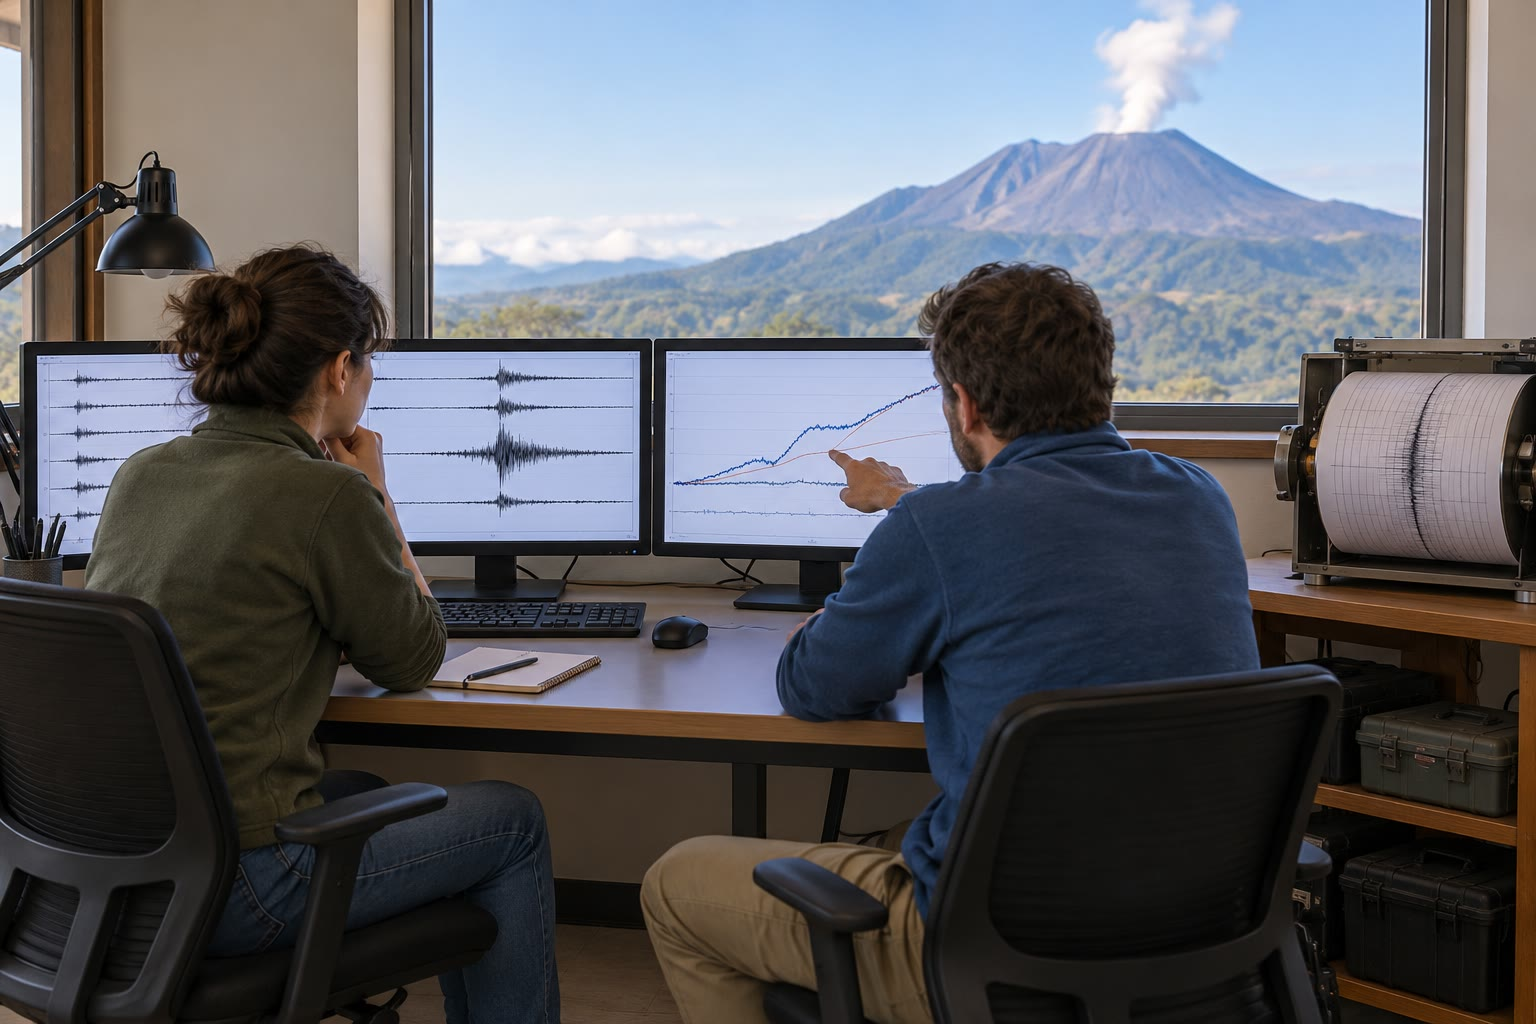
\includegraphics[width=\linewidth]{images/book4/ai/b2-volcano-observatory.jpg}
\par\smallskip{\scriptsize علماء يراجعون سجلّات زلزالية في مرصد
بركاني (رسم توضيحي مولَّد بالذكاء الاصطناعي).}
\end{minipage}
\end{inthefield}
% ledger: hvo:alert-levels

\section{التمارين}

\begin{exercise}[$\star$]\label{exo:b2:eruptive-styles:1}
أعطِ مؤشر VEI الذي يدلّ عليه الحجم الكلي للتيفرا وحده من أجل: (أ) رماد
جبل سانت هيلينز، 18 مايو 1980، \qty{1.3}{km^3}؛ (ب) راسب الطبقة~5 المتساقط من كوتوباكسي،
\qty{0.29}{km^3}؛ (ج) ثوران صغير حجمه \qty{2e6}{m^3}. (د) تُذكر المواد
التي قذفها بيناتوبو في 1991 بأنها «أكثر من \qty{5}{km^3}»، ومع ذلك
صُنّف الثوران VEI~6. ما الحجم الكلي الأدنى الذي يقتضيه هذا التصنيف؟
\end{exercise}
% ledger: usgs:vei-criteria, usgs:msh-1980-ash, biass19:layer5, usgs:pinatubo-1991

\begin{exercise}[$\star$]\label{exo:b2:eruptive-styles:2}
سمِّ كل قطعة فتاتية بركانية: (أ) شظية زجاجية طولها \qty{0.5}{mm}؛ (ب) قطعة
خفاف عرضها \qty{3}{cm}؛ (ج) قطعة زاويّة من حمم قديمة عرضها \qty{20}{cm}؛
(د) كتلة مغزلية الشكل طولها \qty{8}{cm} ملتوية الطرفين.
\end{exercise}
% ledger: nps:pyroclast-sizes

\begin{exercise}[$\star$]\label{exo:b2:eruptive-styles:3}
باستعمال $H = 0.304\,Q^{0.241}$ (حيث $H$ بالكيلومتر فوق المنفذ، و$Q$ بوحدة
\unit{kg/s}): (أ) احسب $H$ من أجل $Q = \qty{e6}{kg/s}$ و\qty{e8}{kg/s}؛
(ب) احسب معدل الثوران الكتلي الذي يقتضيه عمود ارتفاعه \qty{35}{km}،
وشدّته $I = \log_{10}Q + 3$؛ (ج) بأيّ عامل يتغيّر $Q$ إذا كان الارتفاع المقيس
أعلى من الحقيقي بنسبة \qty{20}{\percent}؟
\end{exercise}
% ledger: aubry23:fits, brown14:record

\begin{exercise}[$\star$]\label{exo:b2:eruptive-styles:4}
للراسب المتساقط في الطبقة~5 من كوتوباكسي حجم كلي قدره \qty{0.29}{km^3}. باعتبار
كثافة كلية قدرها \qty{1000}{kg/m^3} للراسب و\qty{2500}{kg/m^3}
للصهارة، احسب حجمه المكافئ للصخر الكثيف، وكتلته ومقداره
$M = \log_{10}m - 7$.
\end{exercise}
% ledger: biass19:layer5, brown14:record

\begin{exercise}[$\star\star$]\label{exo:b2:eruptive-styles:5}
راسب متساقط سمكه \qty{40}{cm} على خط تساوي السمك $\sqrt A = \qty{5}{km}$
و\qty{10}{cm} على الخط $\sqrt A = \qty{15}{km}$، ويرقّ وفق دالة
أسّية واحدة. احسب $k$، و$T_0$، ومسافة تنصيف السمك $\ln 2/k$، والحجم
الكلي، ومؤشر VEI.
\end{exercise}

\begin{exercise}[$\star\star$]\label{exo:b2:eruptive-styles:6}
(أ) بيّن أن الحجم داخل خط تساوي السمك $x = \sqrt A$ لراسب يرقّ
وفق $T_0e^{-kx}$ هو $\frac{2T_0}{k^2}[1 - (1 + kx)e^{-kx}]$. (ب) حلّ $(1 + u)e^{-u} =
1/2$ بثلاثة أرقام معنوية بالتعويض المتكرّر أو بالتنصيف. (ج) من أجل
راسب \cref{exo:b2:eruptive-styles:5}، خارج أيّ خط تساوي سمك يقع نصف الحجم؟ قارن
بالمسافة عن المنفذ لأبعد خط تساوي سمك رُسم.
\end{exercise}

\begin{exercise}[$\star\star$]\label{exo:b2:eruptive-styles:7}
صهارة ريوليتية عند \qty{850}{\celsius} (\qty{1123}{K}) تحوي
\qty{5.0}{\percent} من الماء، ذوبانيته $s = 0.444$ في المئة لكل
$\sqrt{\unit{MPa}}$؛ وكثافة مصهورها \qty{2300}{kg/m^3}. (أ) احسب
ضغط إشباعها، والعمق الذي يُبلغ عنده لتدرّج ضغط
قدره \qty{0.025}{MPa/m}. (ب) احسب الكسر الحجمي للغاز عند
\qty{10}{MPa} إذا بقي الغاز في \omterm{def:b2:magma-emplacement:magma}{الصهارة} ($R = \qty{8.314}{J/(mol.K)}$، $M =
\qty{0.018015}{kg/mol}$). (ج) لماذا تتفتّت الصهارات البازلتية أقل بكثير
مع أن بازلتًا في نظام مغلق فيه \qty{1}{\percent} من
الماء يكون عند \qty{1}{MPa} غازًا بنسبة \qty{92}{\percent}؟
\end{exercise}
% ledger: moore98:h2o, cassidy18:fragmentation, cassidy18:ascent

\begin{exercise}[$\star\star$]\label{exo:b2:eruptive-styles:8}
(أ) يزداد حجم \omterm{prop:b2:eruptive-styles:mogi}{مصدر موغي} على عمق \qty{5}{km} بمقدار \qty{e7}{m^3}. احسب
الرفع فوقه ($\nu = 0.25$). (ب) ينخفض انتفاخ آخر إلى نصف قيمته القصوى
على بعد \qty{3.8}{km} من مركزه: ما عمق مصدره؟ (ج) ما الحصّة من
الرفع الأقصى التي تراها محطة على مسافة أفقية تساوي عمق
المصدر؟
\end{exercise}
% ledger: dmodels:mogi

\begin{exercise}[$\star\star$]\label{exo:b2:eruptive-styles:9}
يقذف انفجار فولكاني كتلًا من فوّهة. بإهمال مقاومة الهواء
وارتفاع حافة الفوّهة، احسب أكبر مدى لكتلة مقذوفة
بسرعة \qty{100}{m/s}، ثم \qty{200}{m/s} ($g = \qty{9.81}{m/s^2}$). هل تجعل مقاومة
الهواء هذين المديين حدًّا أعلى أم أدنى؟ ولماذا يتناسب نطاق
خطر المقذوفات حول المنفذ مع مربع سرعة الإطلاق؟
\end{exercise}

\begin{exercise}[$\star\star\star$]\label{exo:b2:eruptive-styles:10}
(أ) استنتج حجم راسب ذي مقطعين أسّيين المعطى في
إطار الطريقة، مفترضًا أن السمك متصل حيث يتقاطع المستقيمان. (ب) من أجل
راسب الطبقة~5 المتساقط من كوتوباكسي، المقطعان المضبوطان هما $T = \qty{1285}{cm}\times
e^{-0.365x}$ ومقطع بعيد ميله $k_2 = \qty{0.138}{km^{-1}}$، يتقاطعان عند
$X = \qty{8.56}{km}$. احسب الحجم، وحصّته الواقعة خارج نقطة
التقاطع.
\end{exercise}
% ledger: biass19:layer5

\begin{exercise}[$\star\star\star$]\label{exo:b2:eruptive-styles:11}
(أ) باستعمال \cref{prop:b2:eruptive-styles:plume}، بأيّ عامل يزداد ارتفاع
العمود حين يُضرب معدل الثوران في 100؟ قارن بالأسّين
التجريبيين $0.241$ و$0.226$. (ب) في أيّ اتجاه يغيّر غلاف جوي أشدّ
تطبّقًا الارتفاعَ، وبكم إذا ازداد $N$ بنسبة
\qty{20}{\percent}؟ (ج) أعطِ سببين قد يجعلان الأسس المقيسة أدنى من
$1/4$.
\end{exercise}
% ledger: aubry23:fits

\begin{exercise}[$\star\star\star$]\label{exo:b2:eruptive-styles:12}
يُدرج الفهرس العالمي 132 ثورانًا من VEI~4 أو أكثر بدأت بين 1500
و1899، و95 بين 1900 و2024. (أ) احسب المعدل في القرن في كل
فترة. (ب) إذا كان المعدل منذ 1900 هو الحقيقي، فما الحصّة المسجّلة من الثورانات
الأقدم؟ (ج) تجد دراسة للثورانات الكبيرة 21 ثورانًا
مقدارها من 4 إلى 4.9 في القرن بين 1500 و1900 و56 منذ 1900؛ قارن.
(د) لماذا تتوقف هذه الحصّة على حجم الثورانات؟
\end{exercise}
% ledger: data:b4-gvp-eruptions, brown14:record

\section{مسألة: قراءة راسب بليني}

\begin{problem}[{مسألة نهاية الأسبوع --- من خطوط تساوي السمك لراسب خفاف متساقط إلى حجم
ثورانه، وارتفاع عموده، وكم مرة تحدث مثل هذه
الثورانات}]
\label{pb:b2:eruptive-styles:1}
خلّف بركان متخيَّل راسب خفاف متساقطًا من طور بليني واحد
دام \qty{10}{\hour}. وخطوط تساوي سمكه، بعد إزالة استطالة الريح
باستعمال الجذر التربيعي لمساحاتها، هي:
\begin{center}
\small
\begin{tabular}{lccccc}
\hline
\mbox{\textdir TLT $\sqrt A$ (\unit{km})} & 10 & 20 & 40 & 80 & 120 \\
السمك \mbox{\textdir TLT $T$ (\unit{cm})} & 200 & 100 & 48 & 14 & 4.0 \\
\hline
\end{tabular}
\end{center}
البيانات: الكثافة الكلية للراسب \qty{900}{kg/m^3}؛ كثافة \omterm{def:b2:magma-emplacement:magma}{الصهارة}
\qty{2400}{kg/m^3}؛ ارتفاع العمود المقيس من أكبر القطع،
\qty{31}{km} فوق المنفذ؛ التروبوبوز عند \qty{16}{km}. استعمل $H =
0.304\,Q^{0.241}$ و$H = 0.345\,Q^{0.226}$ (حيث $H$ بالكيلومتر، و$Q$ بوحدة
\unit{kg/s}).

\medskip\noindent\textbf{الجزء الأول --- الراسب.}
\begin{enumerate}
\item احسب $\ln T$ لكل خط تساوي سمك وبيّن أن النقاط تقع على مقطعين
مستقيمين حين تُرسم بدلالة $\sqrt A$. أين الانكسار؟
\item احسب الميل $k_1$ والجزء المقطوع $T_0$ للمقطع القريب
المارّ بخطّي تساوي السمك الأوّلين.
\item مستقيم المربعات الصغرى المارّ بخطوط تساوي السمك البعيدة الثلاثة هو $T =
\qty{167}{cm}\times e^{-0.0311\sqrt A}$. تحقّق من أنه يمرّ في حدود
\qty{5}{\percent} من كلٍّ منها.
\item احسب قيمة $\sqrt A$ التي يتقاطع عندها المستقيمان.
\item احسب مسافتَي تنصيف السمك $\ln 2/k$ للمقطعين.
\item احسب الحجم الذي كان سيكون للراسب لو رقّ بميل المقطع القريب
في كل مكان.
\item احسب الحجم الكلي بالمقطعين، والحصّة التي يسهم بها
تصحيح المقطع البعيد الألطف ميلًا.
\item بأيّ عامل كان الحجم سيُقدَّر بأقل من قيمته لو لم يُرسم إلا الراسب
القريب؟ ولماذا يمثّل هذا خطرًا حقيقيًا في الرواسب القديمة؟
\end{enumerate}

\noindent\textbf{الجزء الثاني --- حجم الثوران.}
\begin{enumerate}[resume]
\item أعطِ مؤشر VEI للثوران.
\item احسب الحجم المكافئ للصخر الكثيف.
\item احسب الكتلة المقذوفة.
\item احسب المقدار $M = \log_{10}m - 7$.
\item كم مرة يفوق هذا الراسب حجم الرماد المتساقط من جبل سانت هيلينز في 1980،
\qty{1.3}{km^3}؟
\item ما ارتفاع العمود الذي يقرنه جدول VEI بهذا الثوران،
وأيّ طراز؟
\end{enumerate}

\noindent\textbf{الجزء الثالث --- العمود.}
\begin{enumerate}[resume]
\item احسب متوسط معدل الثوران الكتلي على مدى الطور البليني،
وشدّته $I = \log_{10}Q + 3$.
\item احسب ارتفاع العمود الذي يتنبّأ به القانون التجريبي الأول.
\item السؤال نفسه بالقانون الثاني.
\item قارن بالارتفاع \qty{31}{km} المقيس من القطع، مع مراعاة تشتّت
القانونين.
\item ما معدل الثوران الكتلي الذي يقتضيه ارتفاع \qty{31}{km} حسب القانون الأول؟ بأيّ
عامل يختلف عن معدل السؤال~15، وما الذي قد يفسّر ذلك؟
\item هل حقن العمود غازًا في الستراتوسفير؟ ماذا قد يترتّب على ذلك في
المناخ، وما الغاز الأساسي؟
\end{enumerate}

\noindent\textbf{الجزء الرابع --- كم مرة؟}
\begin{enumerate}[resume]
\item من أعداد الفهرس (399 ثورانًا من \mbox{\textdir TLT VEI $\ge 3$} من 1950 إلى
2024، و95 من \mbox{\textdir TLT VEI $\ge 4$} منذ 1900، و22 من \mbox{\textdir TLT VEI $\ge 5$} منذ 1800، و8 من \mbox{\textdir TLT VEI $\ge 6$} منذ
1500، وكل النوافذ تنتهي في 2024 ضمنًا)، احسب المعدلات السنوية الأربعة
ولوغاريتماتها.
\item تحقّق من أن المستقيم $\log_{10}\lambda_v = 3.28 - 0.85\,v$ يمرّ في حدود
\qty{10}{\percent} من كل معدل.
\item لماذا تبدأ كل نافذة أبعد في الماضي للثورانات الأكبر؟
\item من المستقيم، احسب معدل ثورانات \mbox{\textdir TLT VEI $\ge 5$}، ومتوسط
فترة عودتها، واحتمال ثوران واحد على الأقل في السنوات العشر المقبلة.
\item من المستقيم، احسب معدل ثورانات \mbox{\textdir TLT VEI $\ge 7$} وقارنه
بالثورانين المسجّلين منذ العام 1000.
\item من المستقيم، احسب معدل ثورانات \mbox{\textdir TLT VEI $\ge 6$}
واحتمال ثوران واحد على الأقل، بالنسبة المئوية، في مكان ما على الأرض خلال المئة سنة
المقبلة، وهو الرقم الأساسي في هذه المسألة. على أيّ افتراض يستند؟
\end{enumerate}
\end{problem}
